
\noindent
This chapter details the methodological framework employed to investigate physio-adaptive flow detection. Following a \textbf{mixed-method design} \autocite{creswell2017research}, integrates qualitative insights from semi-structured interviews with athletes and industry experts with the technical implementation with the technical implementation of a computational model. In a sequential triangulation design, the methods are not conducted in isolation; rather, the output of the qualitative strand (Phase 1) serves as the foundational input for the development of the technical solution (Phase 2), which is then validated through user-centric testing (Phase 3). This approach ensures that the resulting machine learning (ML) models are not only technically accurate but are built upon the \enquote{ground truth} of the lived experiences of e-sports practitioners. The study follows a three-phase progression, moving from theoretical discovery to practical application and final assessment. As illustrated in Figure~\ref{fig:sequentialTriangulation}, the findings from the initial requirement definition inform the implementation of the problem solution, which is subsequently integrated during the final evaluation.

\begin{figure}[htbp]
    \centering
    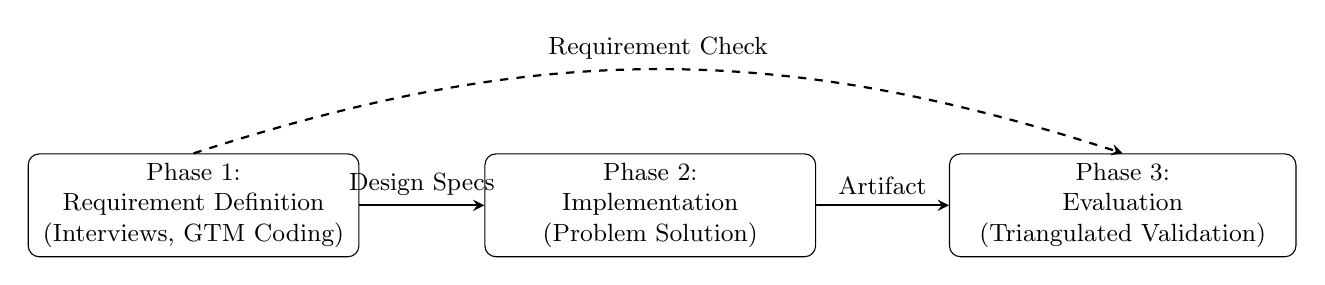
\begin{tikzpicture}[>=stealth, every node/.style={font=\small}]
        \node[draw, rounded corners, minimum width=4.2cm, minimum height=1.1cm, align=center] (qual) at (0,0) {Phase 1:\\Requirement Definition\\(Interviews, GTM Coding)};
        \node[draw, rounded corners, minimum width=4.2cm, minimum height=1.1cm, align=center] (quan) at (5.8,0) {Phase 2:\\Implementation\\(Problem Solution)};
        \node[draw, rounded corners, minimum width=4.4cm, minimum height=1.1cm, align=center] (intg) at (11.8,0) {Phase 3:\\Evaluation\\(Triangulated Validation)};

        \draw[->, thick] (qual) -- node[above] {Design Specs} (quan);
        \draw[->, thick] (quan) -- node[above] {Artifact} (intg);
        \draw[->, dashed, thick, bend left=18] (qual.north) to node[above] {Requirement Check} (intg.north);
    \end{tikzpicture}
    \caption{Sequential triangulation design used in this study: requirement definition, implementation/problem solution, and evaluation.}
    \label{fig:sequentialTriangulation}
\end{figure}

The phases are defined as follows:

\begin{enumerate}
    \item \textbf{Phase 1: Requirement Definition (Qualitative Discovery):} Through semi-structured interviews and a review of the literature, the specific triggers and inhibitors of flow in e-sports are identified. This phase uses Grounded Theory Methodology (GTM) to analyze the data, providing the specific functional requirements for a Physio-Adaptive system \autocite{recker2021researchmethods}.
    
    \item \textbf{Phase 2: Implementation (Problem Solution):} In this phase, the physio-adaptive prototype is developed to address the requirements identified in Phase 1. This involves building the machine learning pipeline (using secondary datasets) and the adaptation layer. The focus here is on the technical creation of a solution that can maintain the flow of the athletes.
    
    \item \textbf{Phase 3: Evaluation (Qualitative Validation):} The completed system is assessed via user testing and a second round of interviews. This final step compares the system's objective classification performance against the user's subjective experience. The goal is to determine if the implemented solution actually meets the requirements defined in the initial qualitative phase.
\end{enumerate}

\subsection{Requirement definition: Semi-Structured Interviews}



\subsubsection{Sampling and Participant Recruitment}
To ensure a focused analysis of flow support in a realistic competitive setting, this study uses a purposive, stratified sampling strategy focused on the LoL competitive ecosystem and on expert knowledge relevant to game-adjacent adaptation. The resulting requirements are \textbf{not} treated as universally valid for all e-sports players. Instead, they are interpreted as design-oriented requirements for a physio-adaptive prototype in the context of competitive LoL.

To establish a triangulated requirements baseline, the qualitative sample consists of three complementary cohorts and a total of nine semi-structured interviews ($N = 9$):
\begin{enumerate}
    \item \textbf{Competitive active players ($n = 3$):} Players provide first-hand accounts of gameplay flow, stress, interruptions, and competitive routines.
    \item \textbf{Game design experts ($n = 3$):} Experts assess whether the proposed adaptive measures are compatible with game mechanics, interface design, pacing, player agency, and competitive integrity.
    \item \textbf{Physiological computing experts ($n = 3$):} Experts assess the technical and methodological plausibility of sensor fusion, real-time data processing, and biocybernetic feedback loops.
\end{enumerate}

The primary player target group is defined as \textbf{Tier 2: high-ELO and semi-professional players}. This group is selected because it combines high competitive pressure and advanced game knowledge with more realistic accessibility for interviews and prototype testing than fully professional Tier 1 players. 

\begin{itemize}
    \item \textbf{Target Player Groups and Stratification:} Participants are categorized into three distinct tiers based on their standing within the official LoL competitive ladder, which comprises the ranks of \textit{Iron, Bronze, Silver, Gold, Platinum, Emerald, Diamond, Master, Grandmaster,} and \textit{Challenger} \autocite{gong2020league}. The stratification is not intended to give all tiers equal authority over the final requirements. Instead, requirements are weighted according to their relevance for the Tier 2 target context:
    \begin{enumerate}
        \item \textbf{Professional Athletes (Tier 1):} Competitors currently active in premier professional leagues such as the \textit{LEC} (EMEA), \textit{LCS} (North America), or the \textit{Prime League Pro Division} (DACH). While players in this tier are almost exclusively ranked in \textit{Challenger}, they are defined by their professional status and contractual obligations. Tier 1 perspectives are used only for contextual orientation where available, but Tier 1 requirements are not inferred from lower-tier participants. \textit{Note: Recruiting within this tier represents a significant methodological challenge due to restricted schedules and strict contracts.}
        
        \item \textbf{High-ELO / Semi-Professional Players (Tier 2):} Highly skilled individuals positioned at the apex of the regional ladder. This group encompasses players in the \textbf{Diamond, Master, Grandmaster,} and \textbf{Challenger} tiers who are not currently active in Tier 1 leagues. These ranks represent the primary target population of the thesis, where the demand for flow-maintenance and the cost of interruptions are expected to be high while access for empirical work remains feasible \autocite{gong2020league}.
        
        \item \textbf{Casual and Intermediate Gamers (Tier 3):} Enthusiasts playing for recreation or amateur-level competition. This group covers the vast majority of the player distribution and includes all individuals ranked from \textbf{Iron, Bronze, Silver, Gold, Platinum,} through to \textbf{Emerald} \autocite{gong2020league}. Tier 3 participants are not used to infer the needs of Tier 1 or Tier 2 players. Their role is strictly to reveal accessibility issues, general usability expectations, and contrasts between casual and advanced competitive play.
    \end{enumerate}

    \item \textbf{Selection Criteria:} Inclusion and exclusion criteria are defined separately for each cohort to make participant selection transparent and comparable across groups:
    \begin{itemize}
        \item \textbf{Competitive Active Players:} Players are included if they are at least 18 years old, actively play LoL, can provide a verifiable \textit{Riot ID} or \textit{Summoner Name}, and currently meet the Tier 2 rank definition. They must also be willing to discuss their competitive setup, communication practices, interruption experiences, and willingness to use an ECG chest belt and webcam in a later prototype evaluation. Players are excluded if their rank cannot be verified, if they are below Diamond at the time of recruitment, if contractual obligations prevent open participation, or if they do not provide informed consent.
        \item \textbf{Game Design Experts:} Game design experts are included if they have worked in game design research or the game industry for at least three years. Eligible experts must have practical or scholarly experience with the design of computer games, including published games, prototypes, research artifacts, or equivalent interactive game projects. The search strategy prioritizes experts who have worked on LoL or comparable multiplayer online battle arena (MOBA) games, because this experience is most relevant for assessing intervention timing, player agency, interface constraints, and competitive integrity. Experts are excluded if their experience is limited to casual game use, if they cannot substantiate relevant game design experience, or if they lack direct professional or scholarly exposure to game mechanics, interface design, or player experience.
        \item \textbf{Physiological Computing Experts:} Physiological computing experts are included if they have worked in physiological computing research or industry for at least three years. Eligible experts must have experience with physiological sensing methods, data acquisition, signal processing, and data-processing workflows, including machine learning pipelines. The search strategy prioritizes experts with experience in ECG or webcam-based measurements, ideally in gaming, entertainment computing, HCI, or other interactive real-time applications. Experts are excluded if their expertise is unrelated to physiological sensing, data acquisition, signal processing, machine learning-based analysis, or human-centered adaptive systems, or if they cannot assess the ethical and practical implications of using physiological signals in an adaptive system.
    \end{itemize}

    \item \textbf{Hardware and Software Context:} Interviews document each participant's relevant setup or professional frame of reference, including computer performance level, monitor configuration, input devices, headset and voice communication setup, operating system environment, and familiarity with ECG or webcam-based sensing. This information is treated as contextual data rather than as a universal technical standard. The prototype is therefore designed for the Tier 2 context and common high-performance gaming setups, not as a guaranteed fit for all professional tournament infrastructures or casual home environments.

    \item \textbf{Recruitment Channels:} Player participants are recruited through university e-sports structures, especially \textit{Uni-Liga} teams at the University of Duisburg-Essen, supplemented by high-ELO community structures such as competitive \textit{Discord} servers and public LoL player forums. Game design experts are contacted through university game design programs, academic faculties at partner art/design universities, professional game development networks, LinkedIn, studio contact pages, and game development directories. Physiological computing experts are contacted through the University of Duisburg-Essen's Entertainment Computing and HCI chairs, research lab websites, publication-based email outreach, and professional networks related to physiological sensing and interactive systems.

    \item \textbf{Verification Procedure:} Player eligibility is verified through the provided \textit{Riot ID} or \textit{Summoner Name} and public ranking or match-history information. Expert eligibility is verified through public institutional profiles, professional profiles, publication records, industry credentials, or self-reported career histories checked for consistency with the inclusion criteria. All participants must provide informed consent before the interview.
\end{itemize}



\subsubsection{Data Collection and Tooling}
Interviews are conducted as semi-structured sessions to allow for emergent themes while ensuring core research questions are addressed. 

\begin{itemize}
    \item \textbf{Interview Platform:} Remote interviews are conducted via \textit{Microsoft Teams} or \textit{Zoom}, utilizing their built-in high-fidelity audio recording features.
    \item \textbf{Transcription:} Initial transcription is performed using \textit{f4transcript}. This software is utilized because it ensures that all data processing and storage occur exclusively on servers located in Germany, adhering to the highest standards of the Federal Data Protection Act (BDSG) and GDPR.
\end{itemize}

\subsubsection{Data Privacy and Ethical Considerations}
In accordance with the General Data Protection Regulation (GDPR), strict privacy standards are maintained throughout the research lifecycle:

\begin{itemize}
    \item \textbf{Informed Consent:} Before the interview, all participants must sign a digital consent form detailing the study's purpose, the nature of data collection, and their right to withdraw at any time without penalty.
    \item \textbf{Data Storage and Security:} All raw audio recordings and transcripts are stored on encrypted, password-protected servers provided by the university. Access is strictly limited to the primary researcher.
    \item \textbf{Anonymization:} Data is pseudonymized immediately following the transcription phase. Real names and identifying details are replaced with alphanumeric codes (e.g., P1-Elite, P2-Casual) to ensure participant privacy during the Grounded Theory analysis.
    \item \textbf{Third-Party Processing:} For automated transcription (Otter.ai), data is uploaded to secure, SOC 2 Type II compliant servers and is permanently deleted from the cloud service once the manual verification phase is complete.
\end{itemize}

\subsubsection{Qualitative Analysis: GTM Coding Workflow}
Following the methodology described by \textcite{recker2021researchmethods}, the analysis utilizes a systematic coding workflow. This process is managed using \textit{MAXQDA} \autocite{MAXQDA2022}, a professional Computer-Assisted Qualitative Data Analysis Software (CAQDAS). 

As a focused application of Grounded Theory Methodology (GTM), this thesis emphasizes coding-based analysis rather than full theory generation. Interview data are iteratively processed through open, axial, and selective coding to derive practically relevant categories for physio-adaptive system design \autocite{recker2021researchmethods,delveholempaecher2024openaxialselective}. In this workflow, open codes are first grouped into higher-order relationships during axial coding (Figure~\ref{fig:axial_coding}), and these relationships are then consolidated into a central explanatory category during selective coding (Figure~\ref{fig:selective_coding}).

The software facilitates the iterative transition between data collection and analysis, allowing for the organized management of \textit{Open}, \textit{Axial}, and \textit{Selective} codes. By utilizing MAXQDA's creative coding and visual mapping tools, the researcher can more effectively identify the "Core Category" that defines the e-sports flow experience, ensuring a rigorous application of the GTM procedures as outlined by \textcite{recker2021researchmethods}.

\begin{figure}[H]
    \centering
    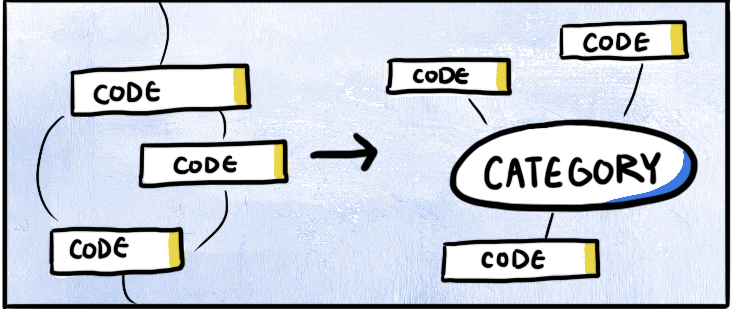
\includegraphics[width=0.9\textwidth]{AxialCoding_DelveTool_2.png}
    \caption{Example of creating axial codes from open codes (Source: \autocite{delveholempaecher2024openaxialselective}).}
    \label{fig:axial_coding}
\end{figure}

\begin{figure}[htbp]
    \centering
    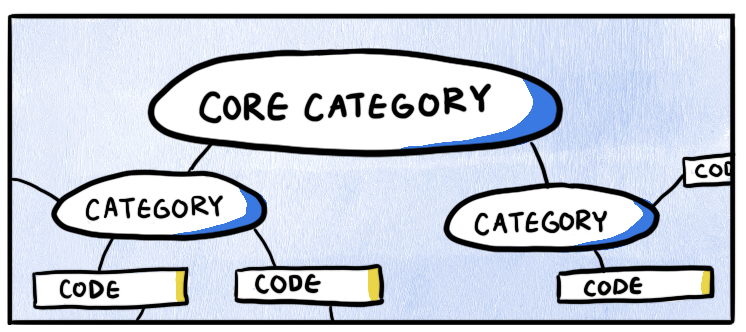
\includegraphics[width=0.9\textwidth]{SelectiveCoding_DelveTool.png}
    \caption{Example of creating selective code from axial codes (Source: \autocite{delveholempaecher2024openaxialselective}).}
    \label{fig:selective_coding}
\end{figure}


\begin{itemize}
    \item \textbf{Open Coding:} Transcripts are broken down into discrete "incidents." Codes such as "Environmental Distraction," "Cognitive Tunneling," and "Post-interruption Frustration" are assigned.
    \item \textbf{Axial Coding:} Concepts are reassembled to identify relationships. For example, the code "Digital Pings" may be linked as a causal condition to the category "Flow Breakage."
    \item \textbf{Selective Coding:} A central core category, such as \enquote{User-Centric Requirements for Physio-Adaptive Flow Support,} is identified. This category integrates the previously identified inhibitors and facilitators to explain the overarching conditions under which an e-sports athlete accepts or rejects autonomous system interventions. By centering the analysis on these requirements, the qualitative strand provides a direct blueprint for the technical implementation in the subsequent phase.
\end{itemize}

\subsection{Implemention: Computational Experimentation}

\subsubsection{Secondary Data Sources}
Rather than collecting primary physiological data for model training, this thesis conducts a secondary analysis of two labeled physiological datasets. The datasets were selected because they serve complementary roles in the model-development strategy: BIRAFFE2 provides the gaming-oriented basis for multimodal state detection, whereas the Irshad et al. / PhySF dataset offers an additional flow-specific physiological reference dataset. To make the two sources comparable, the shared training space is restricted to the physiological modalities available in both datasets, namely \textbf{EEG, ECG, and EDA}. Webcam-based facial data is considered only in BIRAFFE2-derived models, because the Irshad et al. dataset does not include webcam images or facial video recordings.
\begin{enumerate}
    \item \textbf{BIRAFFE2 Dataset \autocite{kutt2022biraffe2}:}
    \begin{itemize}
        \item \textbf{Selection Rationale:} BIRAFFE2 was selected because it captures affective responses in a gaming context and therefore provides high relevance for the gaming-oriented model-development track. Its main advantage is its \textbf{multimodal scope}: physiological signals are synchronized with gamepad telemetry and \textbf{video-based facial expressions}. This makes it possible to examine internal physiological patterns alongside external behavioral and visual indicators of player state.

        \item \textbf{Dataset Context and Available Modalities:} Participants completed affective gaming tasks, such as a \textit{Space Invaders} clone, while multiple synchronized data streams were recorded. The available BIRAFFE2 data includes physiological signals (\textbf{EEG, ECG, and EDA}), visual and behavioral data (\textbf{webcam-based facial recordings/photos} and \textbf{full gameplay screencasts}), and physical interaction metrics (\textbf{gamepad telemetry}).

        In the comparative model-development strategy, BIRAFFE2 is treated as the basic dataset because it contains both the shared physiological modalities and the additional webcam-based facial data. The BIRAFFE2-derived models therefore define the full multimodal benchmark as well as the ECG--webcam deployment-oriented prototype path. For cross-dataset comparison, however, the physiological feature space remains limited to \textbf{EEG, ECG, and EDA}, since these modalities also exist in the Irshad et al. / PhySF dataset.

        \item \textbf{Ground Truth Strategy:} The primary ground truth is derived from the \textbf{GEQ Core Module} \autocite{ijsselsteijn2013game}, a standardized instrument for evaluating game experience across seven components. For flow-state labeling, this thesis uses the \textbf{Flow subscale}, which consists of five items:
        \begin{enumerate}
            \item Item 3: \enquote{I forgot everything around me.}
            \item Item 12: \enquote{I was fully occupied with the game.}
            \item Item 18: \enquote{I lost track of time.}
            \item Item 25: \enquote{I felt completely absorbed.}
            \item Item 33: \enquote{I was deeply concentrated in the game.}
        \end{enumerate}
        Each item is rated on a 5-point Likert scale (0 = \textit{not at all} to 4 = \textit{extremely}). The flow label is generated by calculating the mean score across these items. High-fidelity flow states are identified when this mean exceeds a defined threshold (e.g., $>3.0$), enabling a direct mapping between physiological patterns and the subjective dimensions of immersion, absorption, and concentration.
    \end{itemize}

    \item \textbf{Irshad et al. Dataset \autocite{irshad2023wearable}:}
    \begin{itemize}
        \item \textbf{Selection Rationale:} The Irshad et al. / PhySF dataset was selected because it was specifically curated for flow recognition with consumer-grade and research-grade wearable sensors. It therefore complements BIRAFFE2 by providing a flow-focused physiological benchmark and by reflecting the type of non-invasive sensing that is relevant for home, training, or facility-based e-sports settings.

        \item \textbf{Dataset Context and Available Modalities:} The PhySF dataset used by Irshad et al. was collected during work-related tasks and is used for binary flow recognition rather than for modeling boredom, flow, and stress as three separate target states. Participants first completed a baseline recording and then performed mathematical and reading tasks while multimodal physiological signals were recorded. The dataset combines three hardware devices: an \textbf{EMOTIV Insight} headset for EEG, an \textbf{Empatica} wristband for PPG, infrared thermopile skin temperature, and EDA, and a \textbf{Biosignalsplux RespiBAN} chest wearable for respiration, EOG, ECG, and EMG \autocite{irshad2023wearable}. Importantly, this dataset does \textbf{not} contain webcam images or facial video data; it contributes strictly wearable physiological signals to this thesis \autocite{irshad2023wearable}.
        
        \item \textbf{Ground Truth Strategy:} The ground truth in the Irshad et al. dataset is not based on the \textit{Flow Short Scale (FSS)} and is not collected through continuous in-task self-reporting, because such interruptions would disturb the target state. Instead, task recordings are retrospectively segmented using participants' post-task self-reports. After each task, participants indicated whether they had experienced flow and, if so, in which third of the task the flow episode occurred \autocite{irshad2023wearable}. Physiological windows from the reported flow interval are labeled as \textit{flow}, whereas the remaining task windows and recordings without reported flow are labeled as \textit{non-flow}. This produces temporally localized binary labels for flow/no-flow classification rather than continuous questionnaire scores \autocite{irshad2023wearable}.
    \end{itemize}
\end{enumerate}


\noindent
Based on this modality overlap, four model combinations are trained and compared:
\begin{enumerate}
    \item \textbf{BIRAFFE2 full multimodal model:} EEG, ECG, EDA, and webcam-based facial data.
    \item \textbf{Irshad/PhySF full physiological model:} EEG, ECG, and EDA without webcam data, because the dataset contains no webcam images.
    \item \textbf{BIRAFFE2 deployment-oriented model:} ECG and webcam-based facial data, matching the planned live prototype hardware.
    \item \textbf{Irshad/PhySF deployment-oriented baseline:} ECG-only physiological features, because the dataset has ECG but no webcam data.
\end{enumerate}
This structure preserves the available modality descriptions of each dataset while making clear which features are actually used for model training and which model paths are dataset-specific.

\subsubsection{The Machine Learning Pipeline}
The development and optimization of the supervised learning pipeline are implemented in \textit{Python 3.9}. This specific version was selected to ensure a stable execution environment with broad compatibility for the complex dependency trees of high-level physiological libraries, avoiding the experimental instability of newer releases while maintaining support for modern asynchronous processing.

The model-development process explicitly distinguishes between dataset-specific full and deployment-oriented configurations to separate offline benchmarking from practical runtime capabilities. The full benchmark tracks use the overlapping physiological modalities \textbf{EEG, ECG, and EDA} in both datasets; webcam-based affect features are added only for BIRAFFE2. The deployment-oriented tracks use the signals that can inform the planned prototype path: \textbf{ECG + webcam} for BIRAFFE2 and \textbf{ECG only} for Irshad/PhySF. Additional modalities available in the source datasets (e.g., gamepad telemetry in BIRAFFE2; Respiration, EOG, and EMG in the Irshad dataset) are excluded because they are either structurally incompatible with LoL's mouse-and-keyboard setting or highly susceptible to movement and voice-chat artifacts in e-sports.

Figure~\ref{fig:classification_pipeline} summarizes the complete classification workflow from the two secondary datasets to real-time flow/non-flow prediction. It makes the dataset-specific deployment paths explicit: BIRAFFE2 can feed the ECG--webcam prototype model, whereas the Irshad et al. / PhySF dataset can only feed an ECG-only deployment baseline because it contains no webcam recordings.

\begin{figure}[htbp]
    \centering
    \resizebox{0.96\linewidth}{0.68\textheight}{%
    \begin{tikzpicture}[
        >=stealth,
        % Global node distances (vertical and horizontal)
        node distance=1.25cm and 1.55cm, 
        every node/.style={font=\scriptsize},
        process/.style={draw, rounded corners, align=center, text width=3.15cm, minimum height=1.15cm, inner sep=5pt},
        decision/.style={draw, rounded corners, align=center, text width=3.35cm, minimum height=1.15cm, inner sep=5pt, fill=gray!10},
        dataset/.style={draw, rounded corners, align=center, text width=3.35cm, minimum height=1.15cm, inner sep=5pt, fill=gray!5},
        model/.style={draw, rounded corners, align=center, text width=3.65cm, minimum height=1.3cm, inner sep=5pt, fill=gray!5}
    ]
        % --- ROW 1 (Forward Path) ---
        \node[process] (raw) {Raw Dataset\\Signals};
        \node[dataset, right=of raw] (biraffe) {BIRAFFE2\\ECG, EEG, EDA, Webcam};
        \node[process, right=of biraffe] (prep) {Preprocessing\\Artifact Removal};
        \node[process, right=of prep] (window) {Windowing\\60 s Window / 30 s Step};

        % --- ROW 2 ---
        % Placed directly below BIRAFFE2
        \node[dataset, below=of biraffe] (irshad) {Irshad/PhySF\\Wearables, No Webcam};

        % --- ROW 3 (Return Path) ---
        % Dropped 2.5cm below Windowing to ensure it clears the Irshad node
        \node[process, below=2.5cm of window] (features) {Feature Extraction\\Dataset-Specific Modalities};
        \node[decision, left=of features] (tracks) {Two Feature Tracks\\Full vs. Deployment-Aligned};
        \node[process, left=of tracks] (training) {Model Training\\and Validation};

        % --- ROW 4 (Deployment Path) ---
        % Selection drops below Training, continuing the flow
        \node[process, below=of training] (selection) {Model Selection\\Accuracy, F1, Latency};
        \node[model, right=of selection] (deploy_b) {BIRAFFE2 Prototype Model\\ECG + Webcam Only};
        \node[process, right=of deploy_b] (prediction) {Real-Time Prediction\\Flow / Non-Flow};

        % --- ROW 5 ---
        \node[model, below=of deploy_b] (deploy_i) {Irshad Deployment Baseline\\ECG Only};

        % --- EDGES ---
        % Forward flow
        \draw[->, thick] (raw) -- (biraffe);
        \draw[->, thick] (raw) |- (irshad);
        \draw[->, thick] (biraffe) -- (prep);
        \draw[->, thick] (irshad) -| (prep);
        \draw[->, thick] (prep) -- (window);
        
        % Return flow (Snake)
        \draw[->, thick] (window) -- (features);
        \draw[->, thick] (features) -- (tracks);
        \draw[->, thick] (tracks) -- (training);
        \draw[->, thick] (training) -- (selection);
        
        % Deployment flow
        \draw[->, thick] (selection.east) -- node[above, font=\tiny, midway] {B2} (deploy_b.west);
        \draw[->, thick] (selection.south) |- node[pos=0.25, right, font=\tiny] {PhySF} (deploy_i.west);
        
        % Prediction flow
        \draw[->, thick] (deploy_b.east) -- (prediction.west);
        % The -| notation draws horizontally then vertically into the bottom of prediction
        \draw[->, thick, dashed] (deploy_i.east) -| (prediction.south);
        
    \end{tikzpicture}
    }
    \caption{Dataset-specific model paths for real-time flow prediction.}
    \label{fig:classification_pipeline}
\end{figure}

\begin{itemize}
\item \textbf{Preprocessing:} Signal cleaning and artifact removal are performed using specialized toolkits to ensure high signal-to-noise ratios. \textit{NeuroKit2} is utilized for ECG and EDA data processing due to its comprehensive suite of built-in filters and peak-detection algorithms designed specifically for bio-signal analysis \autocite{makowski2021neurokit2}. For the EEG data, the \textit{MNE-Python} library is employed; it is widely regarded as the industry standard for electrophysiological data, offering robust methods for Independent Component Analysis (ICA) and automated artifact rejection \autocite{gramfort2013mne}. These tools are essential for removing ocular and muscular artifacts which are particularly prevalent in the high-intensity, active environments characteristic of e-sports.

\pagebreak[3]
\item \textbf{Feature Engineering:} Features are extracted using a fixed \textbf{60-second sliding window} with a \textbf{30-second step size}, resulting in 50\% overlap between consecutive windows. The 60-second window is selected as the primary analysis window because HRV frequency-domain features require a sufficiently long segment to produce stable estimates of LF and HF power, whereas substantially shorter windows would make these measures less reliable. The 30-second step size preserves temporal responsiveness by updating the feature representation twice per minute without discarding the physiological stability gained from the longer window. To avoid data leakage, overlapping windows derived from the same participant recording are never split across training and test sets. Instead, splitting is performed at the participant level during cross-validation, so that all windows from a held-out participant remain exclusively in the test fold. This ensures that the model is evaluated on unseen participants rather than on temporally adjacent windows from the same recording. Table~\ref{tab:feature_mapping} provides a specific overview of the feature sets extracted, explicitly differentiated by their target configuration track.

\begin{table}[!tbp]
    \centering
    \scriptsize
    \caption{Overview of Feature Extraction differentiated by Pipeline Configuration.}
    \renewcommand{\arraystretch}{1.3}
    \begin{tabularx}{\linewidth}{|l|L|L|L|}
        \hline
        \rowcolor{black}
        \textbf{\color{white} Signal Modality} & \textbf{\color{white} Statistical Features} & \textbf{\color{white} Frequency-Domain / Temporal} & \textbf{\color{white} Non-linear Features} \\
        \hline
        \multicolumn{4}{|c|}{\cellcolor{gray!20}\textbf{Deployment-Aligned Configuration (Live Prototype \& Full Multimodal)}} \\
        \hline
        \textbf{ECG (HRV)} & Mean HR, SDNN, RMSSD, pNN50 & LF Power, HF Power, LF/HF Ratio & Sample Entropy (SampEn), Detrended Fluctuation Analysis (DFA) \\
        \hline
        \textbf{Webcam} & Mean and Variance of Emotion Probabilities (Neutral, Happy, Angry); Z-axis Rotation & Eye Fixation Duration Percentage; Micro-Expression Peak Frequencies & Gaze Path Length Complexity; Head Orientation Movement Entropy \\
        \hline
        \multicolumn{4}{|c|}{\cellcolor{gray!20}\textbf{Full Multimodal Configuration Only (Offline Benchmarking)}} \\
        \hline
        \textbf{EEG} & Mean PSD per channel, Band Variance & Theta, Alpha, and Beta Power; Alpha/Theta Ratio & Spectral Entropy, Hurst Exponent \\
        \hline
        \textbf{EDA} & Mean SCL, Max SCR Amplitude, SCR frequency & Power Spectral Density (PSD) of phasic component & Lyapunov Exponent, Signal Complexity \\
        \hline
    \end{tabularx}
    \label{tab:feature_mapping}
\end{table}

The extracted features are categorized into three domains:

\begin{itemize}
    \item \textbf{Statistical Features (Arousal Baseline):} These provide a baseline measure of physiological arousal and capture sudden shifts in engagement. For example, sudden shifts in Mean Heart Rate (ECG) represent acute stress responses to in-game events, while stable Neutral affect probabilities (Webcam) establish an immersion baseline.
    
    \item \textbf{Frequency-Domain / Temporal Features (Balance and Immersion):} For HRV, this includes Low Frequency (LF) power, High Frequency (HF) power, and the LF/HF ratio to capture the complex autonomic dual-branch co-activation patterns that characterize physiological flexibility during flow \autocite{uechtritz2026neurophysiological}. For the full multimodal benchmark, EEG power ratios (Alpha/Theta) are included to characterize the depth of cognitive immersion \autocite{katahira2018eeg}, while EDA contributes frequency-domain descriptors of arousal dynamics. In the final live evaluation, this is restricted to the ECG and Webcam temporal features (e.g., fixation durations).
    
    \item \textbf{Non-linear Features (Signal Complexity):} Measures such as Sample Entropy quantify the complexity and regularity of the signals. In flow states, physiological signals often exhibit more \enquote{efficient} regularity, whereas the chaotic patterns seen in states of high anxiety or \enquote{tilt} result in higher entropy values.
\end{itemize}

   \item \textbf{Classification Models:} The selection of machine learning classifiers is informed by the dual requirements of high accuracy and computational efficiency for real-time applications. Following the technical precedent of \textcite{9296229}, this study adopts a multi-model benchmarking approach. 

Initially, a suite of traditional supervised learning algorithms is employed to establish a performance baseline:
\begin{itemize}
    \item \textbf{Support Vector Machines (SVM):} Utilized for their ability to identify optimal hyperplanes in high-dimensional multimodal spaces. SVMs are particularly effective at handling the margin-based separation between "flow" and "non-flow" when the feature space is extensive.
    \item \textbf{Random Forest (RF) and Gradient Boosting (XGBoost):} These ensemble methods are included as they are robust against outliers and can model non-linear relationships without intensive hyperparameter tuning. Crucially, Random Forest provides \textit{feature importance} rankings, which allow for the interpretability of which specific markers (e.g., HRV time-domain metrics vs. Webcam affect probabilities) are most indicative of flow \autocite{9296229}.
    \item \textbf{k-Nearest Neighbors (k-NN):} A non-parametric baseline used to assess the local cluster density of physiological states in the feature space.
\end{itemize}

To map the complex dynamics of the "Flow Channel," this research additionally evaluates three specific Deep Learning (DL) architectures:

\begin{itemize}
    \item \textbf{Long Short-Term Memory (LSTM):} Selected specifically to address the \textbf{temporal dependency} of flow. Unlike traditional models that treat data windows as independent points, LSTMs utilize a gated memory mechanism to "remember" previous physiological states. An LSTM can detect the \textit{transition} into flow by analyzing the sequence of changes in heart rate variability and emotion probabilities over time.
    
    \item \textbf{Convolutional Neural Networks (CNN):} Chosen for their \textbf{automated feature extraction} capabilities. 1D-CNNs are highly effective at identifying local patterns (morphologies) in raw waveforms. In this thesis, 1D-CNNs are used to detect specific patterns directly in the raw ECG signal from the chest belt without requiring manual derivation of every HRV band.
    
    \item \textbf{Multi-Layer Perceptron (MLP):} Included to model \textbf{non-linear sensor fusion}. The MLP maps the interactions between disparate data sources—for example, evaluating if a specific decrease in heart rate variability interacting with a simultaneous increase in "Neutral" facial affect probabilities outperforms linear baseline models.
\end{itemize}

The final model selection is determined by an empirical comparison of accuracy, F1-score, precision, recall, and \textit{inference latency} across both the full multimodal and deployment-aligned configurations. The full multimodal models provide a comparative benchmark, while the model selected for the prototype must remain compatible with the deployment-aligned ECG--webcam feature space and real-time latency constraints.
\end{itemize}

\subsection{Research Environment: LoL}
To ensure the feasibility of identifying and implementing specific adaptive measures, this study focuses exclusively on the Multiplayer Online Battle Arena (MOBA) title LoL. LoL provides a highly structured competitive environment with distinct gameplay phases that naturally map to the Flow Channel model: the repetitive, skill-dominant \enquote{laning phase} (risk of boredom) and the high-intensity, cognitively demanding \enquote{teamfight} phase (risk of anxiety).

\subsubsection{Data Acquisition: The Riot Games Live Client API}
The primary technical interface for game-state awareness is the \textbf{Riot Games Live Client Data API}. Unlike standard web-based APIs, this interface runs locally on the user's machine, providing real-time JSON-formatted data regarding the active match. This allows the physio-adaptive system to synchronize physiological signals with objective in-game events without violating anti-cheat protocols.

Key data points utilized from the local endpoint (\texttt{https://127.0.0.1:2999/liveclientdata/allgamedata}) include:
\begin{itemize}
    \item \textbf{Player Vitality and Stats:} Real-time monitoring of Health, Mana, and Level to assess current combat pressure.
    \item \textbf{Event Triggers:} Immediate notification of Kills, Deaths, and Objective captures (e.g., Baron or Dragon), which serve as temporal markers for physiological spikes.
    \item \textbf{Game Timing:} Synchronization of the match clock with the sensor timestamps to correlate fixed 60-second feature windows, updated at 30-second intervals, with specific game phases.
\end{itemize}

\subsubsection{Adaptive Measures: Real-Time Cognitive and Tactical Shielding}
Given that the game client itself is a closed system, the \enquote{problem solution} (Phase 2) focuses on adapting the user's immediate interactive ecosystem and peripheral environment to protect the user's flow state from disruption. Moving beyond rudimentary operating-system-level notification suppression---which competitive athletes may already manage manually---the adaptation engine targets context-aware adjustments outside the protected game client, grounded in affective gaming, flow-support, and cognitive-load-oriented interaction design \autocite{ubt_eref88160,9296229,irshad2023wearable}. The following measures are identified as actionable intervention categories for a prototype evaluation:

\begin{enumerate}
    \item \textbf{External Visual Shielding:} Rather than modifying the in-game HUD, the prototype manages only game-external visual stimuli, such as system notifications, companion dashboards, stream overlays, or secondary-monitor content. When the multimodal classifier detects high cognitive load during critical match phases identified through the local game-state data, non-essential external visual elements can be hidden, dimmed, or delayed. This reduces avoidable visual noise while preserving the integrity of the official game client.
    
    \item \textbf{Intelligent Acoustic Partitioning:} To prevent auditory overload without interfering with vital team communication, the prototype can apply operating-system-level audio rules to external applications. When real-time physiological metrics indicate peak cognitive load during combat events, background applications such as music players can be attenuated, while communication channels and in-game audio remain under the player's control. This keeps the intervention technically feasible and avoids altering competitive game information.
    
    \item \textbf{Attentional Peripheral Cues:} A potential inhibitor of sustained flow in competitive environments is stress-induced narrowing of attention. When webcam-based affect probabilities indicate elevated frustration or anxiety in combination with an ECG-derived reduction in predicted flow, the system can trigger subtle ambient cues outside the game client, for example through peripheral lighting or a secondary display. These cues are intended as non-intrusive reminders to reset attention without injecting tactical information into the match.
    
    \item \textbf{Context-Aware Information Gating:} To reduce automation surprise and preserve player agency, the intensity and duration of interventions are gated by real-time match-state data and conservative safety rules. Shielding mechanisms are activated only during clearly defined high-load windows, such as active combat or objective contests, and are scaled back during lower-pressure phases such as respawn periods or post-fight transitions. The player can override or disable the interventions at any time.
\end{enumerate}



\subsection{Implementation of the Physio-Adaptive System for E-Sports}
Following the model-development phase, the implementation of the physio-adaptive system is conceptualized as a real-time pipeline that links physiological sensing, state inference, and intervention logic. The implementation targets competitive e-sports scenarios in which rapid context changes and high cognitive load require low-latency adaptation.

\begin{itemize}
    \item \textbf{Input Layer:} Multimodal data streams—specifically \textbf{ECG-derived HRV metrics} from the chest belt and \textbf{facial affect probabilities} from the webcam—are continuously acquired and segmented into 60-second sliding windows with a 30-second step size for near-real-time analysis. This ensures that the input features remain strictly limited to the data provided by the provided hardware, allowing for seamless transition from training on the filtered dataset to the live prototype evaluation.
    \item \textbf{Inference Layer:} The trained classifier predicts flow versus non-flow states for each window and outputs a confidence score used for decision-making.
    \item \textbf{Adaptation Layer:} This layer serves as the intervention engine, where a rule-based controller translates the machine learning model's state predictions into specific adaptive actions. Crucially, the logic governing this layer is \textbf{directly derived from the qualitative requirements established in the first phase of the Sequential Triangulation}. 

    Through the Grounded Theory Methodology (GTM) analysis of semi-structured interviews, specific \textit{inhibitors} and \textit{facilitators} of flow were identified. These qualitative categories (derived via Open, Axial, and Selective coding) define the parameters of the "intelligent notification handling." For example, the decision of which alerts are classified as "non-urgent" and the specific timing of the "shielding" duration are grounded in the participants' lived experiences of competitive pressure. By mapping the GTM-derived user needs to the Adaptation Layer, the system ensures that the biocybernetic intervention is not only technically triggered but also contextually appropriate for e-sports athletes.
    \item \textbf{Safety and Override Mechanism:} To preserve user agency, the system includes manual override options and configurable thresholds for adaptation intensity.
\end{itemize}

In practical terms, the implementation is treated as a prototype architecture that can be integrated into game-adjacent environments (communication overlays, desktop notification managers, or tournament training setups) rather than as a full production deployment.

\subsection{Evaluation of the Adaptive System}
The evaluation of the developed solution follows a qualitative validation approach designed to assess the practical utility and experiential acceptance of the system. Crucially, the success criteria for the evaluation are \textbf{directly mapped back to the design requirements identified in the first phase}, ensuring that the system's performance is judged against the actual needs of e-sports practitioners.

\subsubsection{Interview-Based Evaluation Process}
To assess the system's effectiveness, a second round of \textbf{semi-structured interviews} is conducted, utilizing a hybrid evaluation approach. In the \textbf{live pilot phase}, participants are actively equipped with the \textbf{ECG chest belt} and monitored via the \textbf{webcam} while playing LoL. This setup allows for the direct observation of the system's real-time adaptive behavior and provides a basis for immediate post-game feedback regarding the accuracy of flow detection and the utility of the interventions.

If both dataset-derived classifiers achieve competitive baseline performance during the preceding model-development phase, the live pilot evaluation uses a \textbf{between-subject model allocation}. One half of the physical pilot participants uses the deployment-compatible model trained from the BIRAFFE2 feature space, while the other half uses the deployment-compatible model derived from the \autocite{irshad2023wearable} dataset. Because the Irshad dataset does \textbf{not} contain webcam images, this model variant is limited to the wearable physiological feature space and cannot evaluate the webcam-based component of the prototype. This comparison is only conducted if both models meet predefined minimum criteria for classification performance and inference latency; otherwise, only the stronger deployable model is integrated into the prototype. This conditional design prevents participants from evaluating an evidently non-competitive classifier while still allowing both secondary datasets to inform the evaluation when technically justified.

For participants who are unable to attend the live sessions, a \textbf{video-elicitation methodology} is employed. These interviewees are shown high-fidelity video recordings of a LoL session where the physio-adaptive system was applied to another player. This stimulus includes a visualization of the synchronized physiological data (ECG and webcam-based affect) alongside the system's triggered adaptations. Based on this demonstration, these participants provide their expert feedback on the system's logic and its perceived impact on the gaming experience. This dual approach ensures a robust qualitative evaluation by combining direct user experience with broader expert assessment.

During these interviews, e-sports athletes are presented with the functional logic and adaptive responses of the prototype (e.g., through a demonstration of the system's output or a guided walkthrough of the intervention triggers). The interviews aim to capture the "expert-in-the-loop" perspective, allowing participants to evaluate whether the system's autonomous actions align with their professional experience of competitive play. By using the same semi-structured format as the first phase, the study ensures a consistent dialogue that tracks how the initial requirements have been translated into technical features.

\subsubsection{Triangulation and Validity Strategy}
The validity of the research is established through a triangulation strategy that compares the technical outputs of the implementation with the subjective feedback of the players:

\begin{enumerate}
    \item \textbf{Quantitative Baseline Assessment:} The underlying machine learning models, developed using the secondary physiological datasets in the previous phase, are evaluated using \textit{Leave-One-Subject-Out (LOSO)} Cross-Validation. Standard metrics such as Accuracy, F1-score, AUC, and inference latency are used to verify the objective reliability of the state-inference logic before it is subjected to user evaluation. The BIRAFFE2-derived and Irshad/PhySF-derived deployment-compatible models are compared at this stage. Only models that show competitive performance are admitted to the live pilot evaluation; if both qualify, participants are split approximately evenly between the two model variants.
    
    \item \textbf{Qualitative Requirement Fulfillment:} The primary evaluation of the adaptive system is the \textbf{degree of requirement fulfillment} as determined through the follow-up semi-structured interviews. The evaluation focuses on:
    \begin{itemize}
        \item \textbf{Heuristic Alignment:} Does the system’s adaptive logic accurately address the specific triggers and inhibitors of focus identified by players in the first phase?
        \item \textbf{Perceived Trust and Transparency:} Do the players find the autonomous nature of the adaptation trustworthy, and is the system's behavior clear enough to avoid causing "automation surprise" during a match?
        \item \textbf{Contextual Practical Suitability:} Based on participants' experience in ranked, semi-professional, or professional-adjacent LoL contexts, is the proposed adaptive intervention perceived as useful for structured training, scrims, or tournament-like preparation? Since the study does not deploy the system in official high-stakes tournaments, this criterion assesses perceived transferability and practical plausibility rather than definitive suitability for professional match settings.
    \end{itemize}
\end{enumerate}

By comparing the technical performance metrics of the models with the qualitative feedback from the expert interviews, the study identifies points of convergence or divergence. This ensures that the final evaluation determines whether the system provides a contextually appropriate solution that effectively supports the player's state.